\begin{frame}{Clauser--Horne 1974 Paper}
  \begin{center}
    \tikz\node[draw=red!50, fill=red!10, rounded corners=5pt, drop shadow] {
      \includegraphics[width=0.9\linewidth]{images/ch.png}
    };
    \par\vspace{0.3cm}
    \small \textit{Clauser \& Horne: Experimental Consequences of Objective Local Theories (1974)}
  \end{center}
\end{frame}





\begin{frame}{Clauser--Horne Formulation (1974)}

\begin{itemize}
  \item Defined \textbf{Objective Local Theories (OLT)}:  
        outcomes depend only on hidden variables $\lambda$ and local settings, not on distant settings.  
  \pause
  \item Introduced the \textbf{No-Enhancement Assumption}:  
        detection with a polarizer cannot exceed detection without it.  
  \pause
  \item Showed that this weaker assumption was still enough to make Freedman--Clauser results incompatible with all OLT satisfying it.  
  \pause
  \item Proved that some \textbf{supplementary assumption is necessary}:  
        without no-enhancement, one can build an OLT reproducing quantum predictions.  
  \pause
  \item Revealed the \textbf{detection loophole}:  
        experiments of that era only excluded OLT within the no-enhancement class.  
\end{itemize}

\end{frame}


\begin{frame}{Aspect's Experimental Setups (1980s)}

\begin{minipage}{0.58\textwidth}
\vspace{-2.cm}
\textbf{Experimental Program:}
\begin{itemize}
  \item Systematic tests of Bell inequalities using entangled photons from a calcium cascade.  
  \item Progressively designed to close detection and locality loopholes.  
\end{itemize}

\pause

\textbf{Key Features:}
\begin{itemize}
  \item 1981: High-efficiency source, single-channel polarizers.  
  \item 1982 (Two-channel): Polarizing beam splitters, closed the detection loophole.  
  \item 1982 (Time-varying analyzers): Fast switches, addressed the locality loophole.  
\end{itemize}

\vspace{-0.8cm}

\end{minipage}
\hfill
\begin{minipage}{0.38\textwidth}
  \centering
  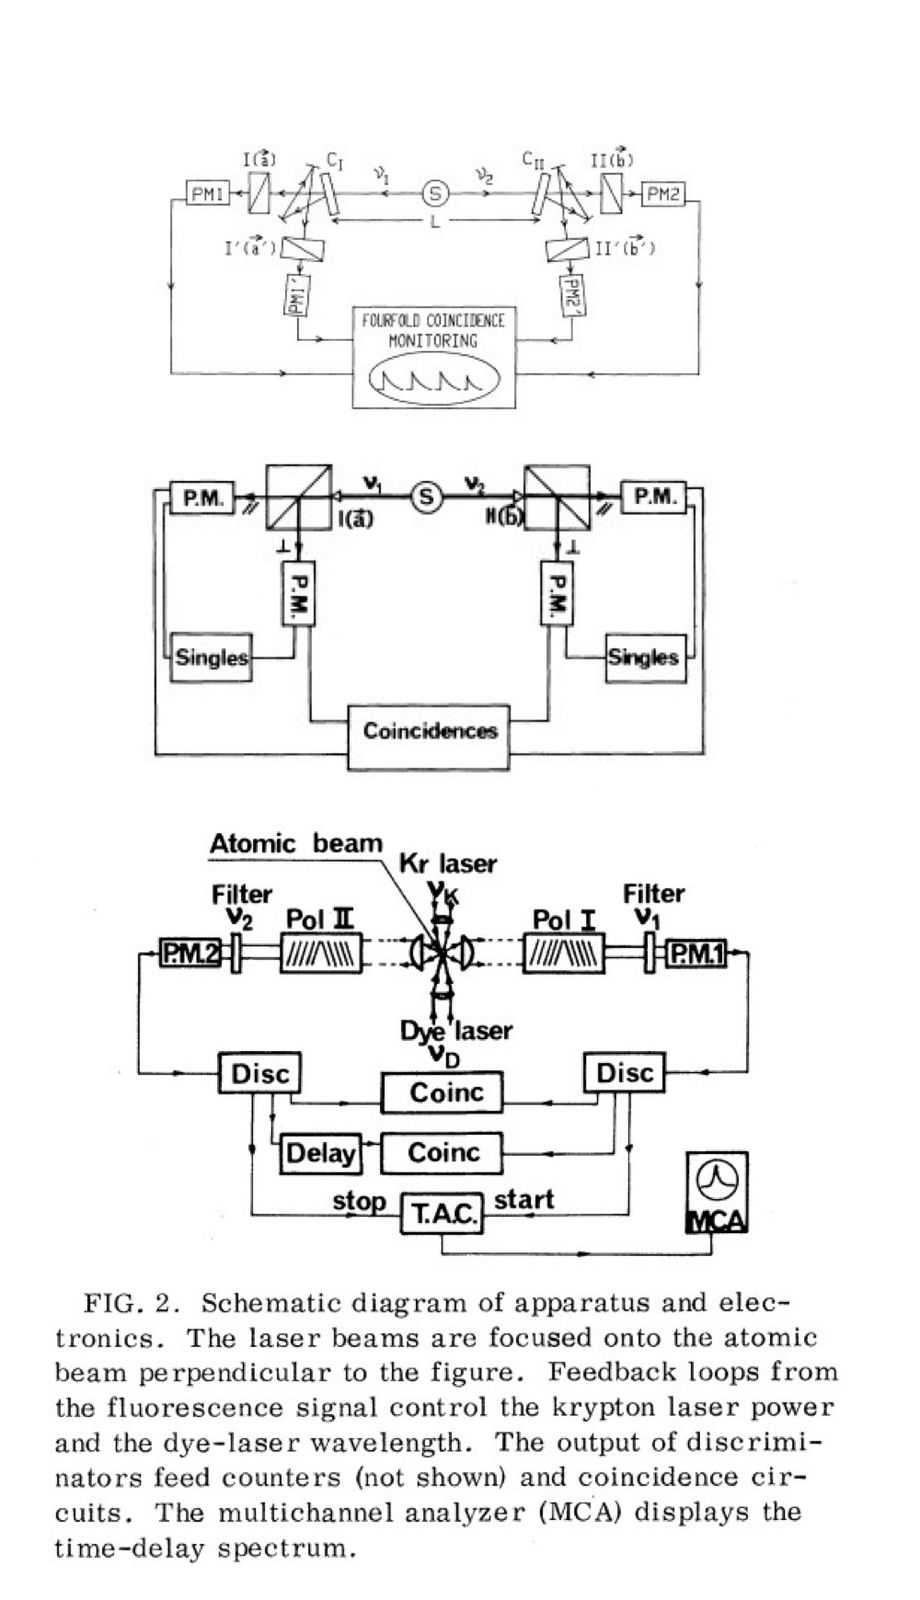
\includegraphics[width=0.8\linewidth]{images/aspect.jpeg} % <--- Imagen del montaje
  \par\vspace{0.2cm}
  \small \textit{Aspect’s photon cascade experiment.}
\end{minipage}

\end{frame}


\begin{frame}{Comparing Aspect’s Three Experiments}

\begin{block}{Progression of Experimental Design}
\begin{itemize}
  \item \textbf{1981:} Improved Freedman–Clauser setup, but still relied on \textit{no-enhancement} assumption (detection loophole).  
  \pause
  \item \textbf{1982 (Two-channel):} Stern–Gerlach–like measurement with PBS. Closed the detection loophole via \textit{fair sampling} assumption.  
  \pause
  \item \textbf{1982 (Time-varying analyzers):} Fast switches ensured space-like separation of choices. Closed the \textit{locality loophole}.  
\end{itemize}
\end{block}

\pause

\begin{center}
  \textbf{Impact:} Each step addressed a loophole, making the violation of Bell’s inequalities increasingly robust and conclusive.  
\end{center}

\end{frame}


